%
% FIX THIS -- remove/change, just some examples of things
%
\chapter{Example chapter}

Example chapter, with apologies to Alex Kolliopoulos,
from whose thesis the examples of math and tables were
borrowed.

\section{Examples of figures and tables}
\label{section:example-figtbl}

This section contains some words, plus
Figure~\ref{fig:xor} and 
Table~\ref{table:treepurpose}.

words, words, words, words,
words, words, words, words,
words, words, words, words,
words, words, words, words,
words, words, words, words,
words, words, words, words,
words, words, words, words,
words, words, words, words,

\begin{figure}[hbtp]
\begin{center}
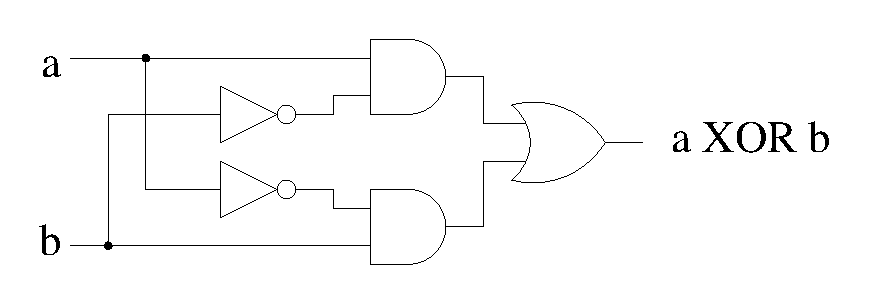
\includegraphics[width=0.5\textwidth]{xor}
\end{center}
\caption{An example figure.}
\label{fig:xor}
\end{figure}

words, words, words, words,
words, words, words, words,
words, words, words, words,
words, words, words, words,
words, words, words, words,
words, words, words, words,
words, words, words, words,
words, words, words, words,

\begin{table}[hbtp]
\begin{tabular}{|l|l|}
\hline 
\textbf{Trial 1} & Expanding a node to select a child\\
\hline
\textbf{Trial 3} & Selecting a node near the middle of a long, linear list\\
\hline
\textbf{Trial 4} & Selecting a node near the top of a long, linear list\\
\hline
\textbf{Trial 5} & Selecting a node near the bottom of a long, linear list\\
\hline
\textbf{Trial 6} & Scrolling and expanding folders in a large tree\\
\hline
\textbf{Trial 7} & Finding a node deep and near the bottom in a large tree\\
\hline
\textbf{Trial 8} & Finding a node near the top of a large tree\\
\hline
\end{tabular}
\caption{Purposes of each experimental trial.}
\label{table:treepurpose}
\end{table}
\section{Examples of math}
\label{section:example-math}

This section contains some math.
First, here's a set of equations.

\begin{eqnarray*}
y_p	&	=	&	\frac{y}{\sqrt{y^2+a^2}}, \\
y_p^2	&	=	&	\frac{y^2}{y^2+a^2}, \\
y_p^2	&	=	&	\frac{y^2+a^2-a^2}{y^2+a^2}, \\
y_p^2	&	=	&	1-\frac{a^2}{y^2+a^2}, \\
y_p^2-1	&	=	&	-\frac{a^2}{y^2+a^2}, \\
1-y_p^2	&	=	&	\frac{a^2}{y^2+a^2}.
\end{eqnarray*}

words, words, words, words,
words, words, words, words,
words, words, words, words,
words, words, words, words,
words, words, words, words,
words, words, words, words,
words, words, words, words,
words, words, words, words,

Now here's a numbered equation.

\begin{equation}
0 = 0 \label{eqn:example}
\end{equation}

\section{Examples of references}

% the "~" makes a no-line-breaks space
Section~\ref{section:example-figtbl} contains 
Figure~\ref{fig:xor} and
Table~\ref{table:treepurpose}.
Section~\ref{section:example-math} contains
Equation~(\ref{eqn:example}).
The sample bibliography file contains references to
an article \cite{pc} and a tech report \cite{opandfunc}, plus some
other things.
% put in bibliography even though not referenced
\nocite{dph}
